%% Section that includes the experiments performed.

This section describes the accomplished experiments that prove how the 
developed system fulfills SKA's requirements for the PPS distribution system. 
\ftglnote{demasiado pretencioso?} The first experiment is a general 
characterization of the PPS distribution system. The second one emulates a 
example of WR network like the one needed to distribute timing in the SKA1-mid, 
and evaluates the synchronization accuracy. Finally, the influence of external 
conditions over the fibre links and its effect on the synchronization accuracy 
is analysed.

The principal equipment and tools utilized to accomplish the presented 
experiments is depicted below:

\begin{itemize}
    \item Two White Rabbit Switches to emulate a two-hops WR network. Both are 
    hardware version 3.4 and are flashed with the last version of the WR 
    firmware (v5.0).
    
    \item A White Rabbit ZEN Time Provider (WR-ZEN TP) to test the performance 
    of the new developed platform as WR nodes of the SKA facilities. The 
    firmware version is 1.2.
    
    \item A High-resolution counter from Keysight, the 52320A.
    
    \item Multiple components for the setup of the equipment:
    \begin{itemize}
        \item Small form-factor pluggable transceptors (SFPs) to stablish the 
        link between WR devices. For the shorter links we've used the most 
        common bidirectional SFPs for WR: AXCEN 1310/1490 nm. For larger links, 
        we tried 
        SFPs from FiberStore: GE-BX-80 1490/1550 nm.
        \item Simplex optical fiber links (G652D). For the device 
        characterization short distance fibres have been used, meanwhile for 
        the scalability and temperature tests we have used long distance links: 
        20 and 50 km respectively.
        \item A OCXO Morion MV89 as frequency reference for the GM mode.
    \end{itemize}
    
\end{itemize}

\subsection{PPS performance of the WR-ZEN platform}
\label{subsec: charact_zen}

With this first experimental results we present a performance analysis of the 
PPS distribution using the WR-ZEN. The connection schema is formed by two 
WR-ZENs, one as WR master and the other as WR slave, whose PPS output signals 
are introduced in a time counter to measure the offset between them. With this 
experiment we focus on the WR-ZEN performance, so that we set all the equipment 
to a constant temperature and we use a short fibre link (few meters) in order 
to avoid instability occasioned by chromatic dispersion on long fibre links.

\begin{table*}\centering
	\ra{0.8}
	\begin{tabular}{@{} rccc@{}}%\toprule
		& MDEV & TDEV (s)  & MTIE (s) \\ \midrule
		\textbf{$\tau$ (s)}\\
		\small{1}     & 2.41868093e-11 & 1.39642609e-11  & 8.78906250e-11 \\
		\small{2}     & 8.18381977e-12 & 9.44986109e-12  & 9.27734375e-11 \\
		\small{4}     & 2.92095805e-12 & 6.74566367e-12  & 1.02539063e-10 \\
		\small{8}     & 1.05378923e-12 & 4.86724395e-12  & 1.02539063e-10 \\
		\small{16}    & 3.70004736e-13 & 3.41795734e-12  & 1.02539063e-10 \\
		\small{32}    & 1.36916757e-13 & 2.52956566e-12  & 1.02539063e-10 \\
		\small{64}    & 5.26969486e-14 & 1.94717424e-12  & 1.02539063e-10 \\
		\small{128}   & 2.41679947e-14 & 1.78603498e-12  & 1.02539063e-10 \\
		\small{256}   & 1.14864284e-14 & 1.69771329e-12  & 1.22070312e-10 \\
		\small{512}   & 6.76882083e-15 & 2.00088603e-12  & 1.22070312e-10 \\
		\small{1024}  & 4.60374214e-15 & 2.72176309e-12  & 1.22070312e-10 \\
		\small{2028}  & 3.37370493e-15 & 3.98911375e-12  & 1.22070312e-10 \\
		\small{4096}  & 1.20303843e-15 & 2.84497740e-12  & 1.31835938e-10 \\
		\small{8192}  & 8.69742436e-16 & 4.11358028e-12  & 1.56250000e-10 \\
		\small{16384} & 			   &                 & 1.66015625e-10 \\
		\small{32768} &				   &                 & 1.66015625e-10 \\
		
		\bottomrule
	\end{tabular}
	\caption{Results of the scalability analysis.}
	\label{tab:exp1res}
\end{table*}

The numerical results are included in Table \ref{tab:exp1res}. Those same 
results are represented graphically on Figures \ref{fig:mdev_exp1}, 
\ref{fig:tdev_exp1} and \ref{fig:mtie_exp1}. The slope of the Modified Allan 
Deviation curve shows that noise is dominated by white phase modulated noise. 
In the time domain, TDEV shows that the expected error is tens of ps and the 
worst-case showed in the MTIE plot is bounded around 200 ps for the sampling 
period. 


\begin{figure}
	\centering
	\begin{subfigure}[t]{0.48\textwidth}
		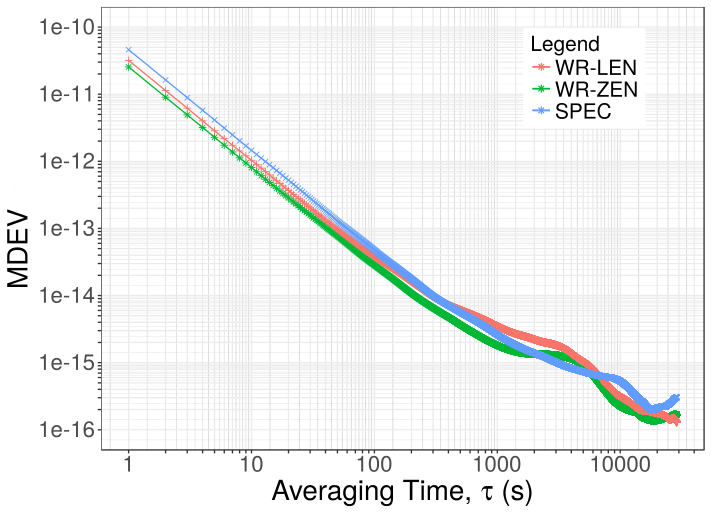
\includegraphics[width=\textwidth]{img/mdev_exp1}
		\caption[MDEV plot for the WR-ZEN]{Modified Allan Deviation plot for a 
		time transfer between two WR-ZEN.}
		\label{fig:mdev_exp1}
	\end{subfigure}
	~ % This symbol adds a white space between images
	\begin{subfigure}[t]{0.48\textwidth}
		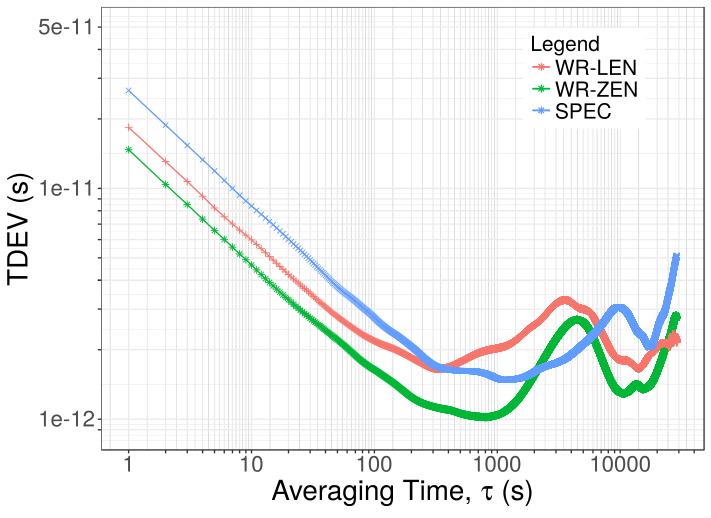
\includegraphics[width=\textwidth]{img/tdev_exp1}
		\caption[TDEV plot for the WR-ZEN]{Time Deviation plot for a time 
		transfer between two WR-ZEN.}
		\label{fig:tdev_exp1}
	\end{subfigure}
	
	\begin{subfigure}[t]{0.48\textwidth}
		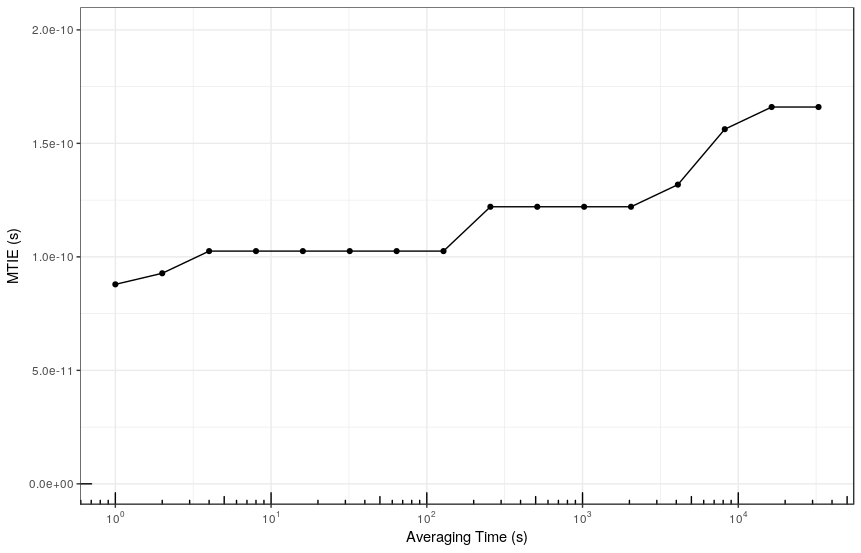
\includegraphics[width=\textwidth]{img/MTIE_exp1}
		\caption[MTIE plot for the WR-ZEN]{Maximum Time Interval Error for a 
		time transfer between two WR-ZEN.}
		\label{fig:mtie_exp1}
	\end{subfigure}
\end{figure}

The obtained values reveal that the proposed PPS distribution system fulfils 
the requirements to be used in the SKA PPS distribution system. Although, it is 
necessary to evaluate the solution in more realistic conditions before 
concluding the goodness of the solution:

\begin{itemize}
	\item Evaluate the WR-ZEN as final node of a WR network. The purpose of 
	this device is to be placed on each acquisition instrument to provide an 
	accurate time reference. The results presented in the subsection 
	\ref{subsec: net_exp} states perfomance for a realistic WR deployment.
	
	\item Moreover, SKA1-mid facilities will be placed in a desert zone, and 
	the nodes will be linked by long-distance fibre links. Because that, it's 
	necessary to analyse if the meteorological conditions can degrade 
	significantly the synchronization accuracy. A thermal characterization of 
	the influence of the variation of propagation delays in the PPS accuracy is 
	presented in subsection \ref{subsec:temp}.
\end{itemize}   

\subsection{WR scalability for SKA} %% Buscar un nombre mejor
\label{subsec: net_exp}

The next experiment covers a scalability analysis of the WR solution for the 
SKA timing system. In section \ref{sec:ska} there is a estimation of the final 
nodes that need to be synchronized for the SKA1-mid: around 250 endpoints that 
must be synchronized with an accuracy below 5ns. A WR network with only two 
hops is suitable to synchronize up to 306 endnodes by the use of WR Switches as 
Boundary Clocks.

We set up a test network composed by a WRS at the top, which is locked to an 
external time reference, another WRS as intermediate BC and a WR-ZEN as 
endpoint. This configuration allows synchronizing up to 306 WR nodes with an 
expected performance similar to the results obtained in our test for the WR-ZEN.

\begin{figure}
	\centering
	\includegraphics[width=0.7\linewidth]{img/prueba_red}
	\caption[WR Scalability test's setup for SKA]{To evaluate the scalability 
	of the WR solution for the expected SKA1-mid timing network, a sample WR 
	network has been evaluated. At the top there's a WRS as GM, a second layer 
	of WRS to finally provide synchronization to the end-nodes (WR-ZEN).}
	\label{fig:pruebared}
\end{figure}


All the equipment for that test was under laboratory conditions. To connect 
each one of the WR devices we've used a 20km fiber spool and SFPs from 
FiberStore (SFP-GE-BX80 with 1490/1550 nm wavelengths). PPS phase difference is 
measured from the WR-ZEN to the WRS in GM configuration using a Keysight 52320A 
counter along 4 hours.

\begin{figure}
	\centering
	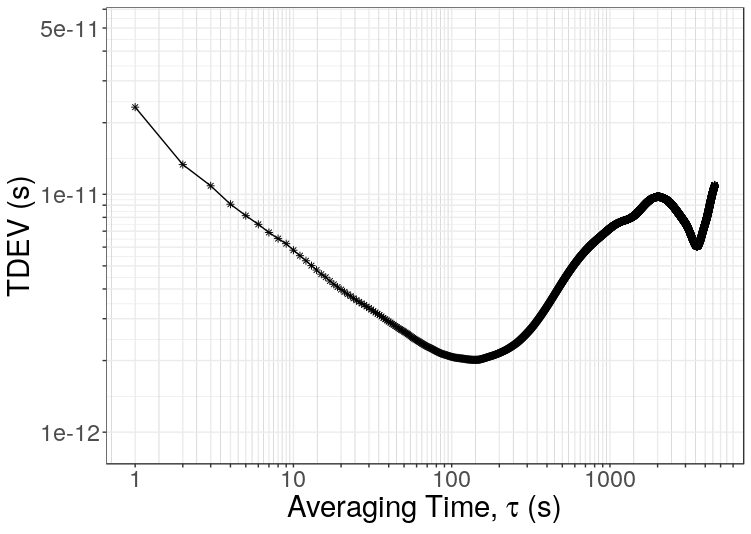
\includegraphics[width=0.9\linewidth]{img/tdev_exp3}
	\caption[TDEV of the end-nodes in the scalability test.]{Time Deviation 
	plot comparing the PPS signal from the end-nodes (WR-ZEN) to the Grand 
	Master of the network.}
	\label{fig:tdevnet}
\end{figure}

TDEV and MTIE values have been calculated by octaves, the numerical values can 
be found in Table \ref{tab:netresults}. Graphical representations are included 
in Figures \ref{fig:tdevnet} and \ref{fig:mtienet} respectively. TDEV results 
show that expected synchronization accuracy for the end-nodes is around tens of 
ps. The maximum PPS error during this test is bounded in hundred of ps, which 
is more than enough what SKA1-mid needs (5ns).

\begin{table*}\centering
	\ra{0.8}
	\begin{tabular}{@{} rcc@{}}%\toprule
		& TDEV (s)  & MTIE (s) \\ \midrule
		\textbf{$\tau$ (s)}\\
		\small{1}     & 2.32509201e-11  & 1.36718750e-10 \\
		\small{2}     & 1.33315382e-11  & 1.36718750e-10 \\
		\small{4}     & 9.08699704e-12  & 1.36718750e-10 \\
		\small{10}    & 5.82194037e-12  & 1.36718750e-10 \\
		\small{20}    & 3.97732795e-12  & 1.36718750e-10 \\
		\small{40}    & 2.91762201e-12  & 1.46484375e-10 \\
		\small{1e2}   & 2.07423753e-12  & 1.46484375e-10 \\
		\small{2e2}   & 2.15075917e-12  & 1.46484375e-10 \\
		\small{4e2}   & 3.37401257e-12  & 1.51367188e-10 \\
		\small{1e3}  & 7.18913143e-12  & 1.66015625e-10 \\
		\small{2e3}  & 9.75471284e-12  & 1.66015625e-10 \\
		\small{4e3}  & 7.54252759e-12  & 1.90429688e-10 \\
		\small{1e4}  &                 & 2.05078125e-10 \\
		
		\bottomrule
	\end{tabular}
	\caption{Results of the scalability analysis.}
	\label{tab:netresults}
\end{table*}

With those results, it's proved that a WR network with two levels can provide 
synchronization to all the equipment expected for the SKA1-mid facilities. 
Although long-distance fiber links have been used for that test, thermal 
influence should be take into account in order to confirm the goodness of the 
WR solution in the SKA timing distribution. The next experiment will evaluate 
how the temperature change in the fiber link can affect the accuracy of the 
synchronization. 


\begin{figure}
	\centering
	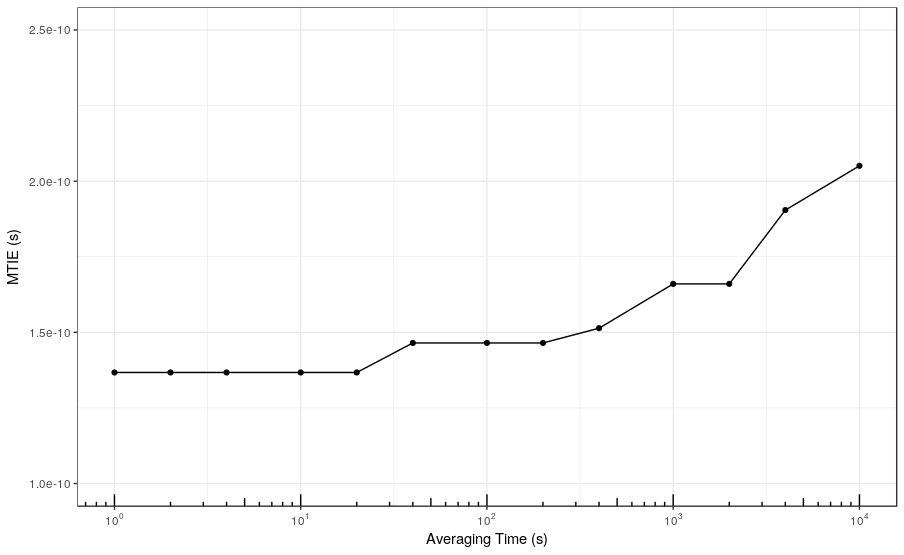
\includegraphics[width=0.9\linewidth]{img/MTIE_exp3}
	\caption[MTIE of the end-nodes in the scalability test.]{Maximum Time 
	Interval Error
	plot comparing the PPS signal from the end-nodes (WR-ZEN) to the Grand 
	Master of the network.}
	\label{fig:mtienet}
\end{figure}

\subsection{Fiber operational temperature influence on time accuracy}
\label{subsec:temp}

One of the key aspects of the timing solution for the SKA facilities is the 
influence evaluation of the external elements in the timing performance. 
Synchronization signals are spread over hundred of nodes which are connected by 
long distance fiber links. Meteorological elements, such as wind or large 
 temperature changes, can alter propagation delays over the fiber 
links. The timing solution must compensate appropriately those effects in order 
to maintain the synchronization performance inside the limits required by the 
SKA's infrastructure.

On this contribution we've focused on the temperature change effect on the cable
\textit{round-trip} time (CRTT) and the PPS performance. To evaluate that, we 
own a climate chamber in the laboratory and some fiber spools of tens of 
kilometers. 
We couldn't evaluate properly wind impact with our equipment, because of this, 
the experiments will only determine temperature effect on synchronization.

\ftgnote{Aquí un párrafo mencionando los efectos físicos sobre los haces de luz 
que viajan por la fibra al cambiar la temperatura. Índice de refracción. 
Aportar referencias!!!!}

Theoretically, WR, is able to dynamically calibrate the master to slave 
propagation delay from the total \textit{round-trip} time, and therefore PPS 
offset shall maintain constant even when the propagation delay changes. The 
accurate estimation of the one-way propagation delay is achieved by the use of 
a constant value, $\alpha$, which express the ratio between propagation times 
with the two wavelengths used in the WR link. A complete explanation of the 
link model could be read in \cite{Wlostowski2011} and \cite{Daniluk2012}.

In the real world, $\alpha$ is temperature dependent, because of the change in 
the refraction index due to a temperature variation in the fiber. For small and 
mid-distance links, in laboratory conditions, $\alpha$ is nearly negligible and 
the current link model behaves very well. The WR network in SKA will be formed 
by long distance links exposed to external elements. In the concrete situation 
of the South Africa facilities, the chosen location was the Karoo region. 
\ftglnote{comprobar eso porque lo he sacado de Wikipedia} This region is a 
semi-desert area, very adequate to reduce human interferences in the high 
resolution data acquisition equipment, but with a inconvenient respec to the 
temperature point of view: desertic zones have a high difference between day 
and night temperatures.

\begin{figure}
	\centering
	\includegraphics[width=0.7\linewidth]{img/tempsetup}
	\caption[Configuration of the climate chamber experiments]{Experimental 
		setup to analyze the influence of the temperature gradient over the 
		fiber 
		link and the synchronization accuracy.}
	\label{fig:tempsetup}
\end{figure}

We performed a series of experiments introducing a 50 km length fiber spool in 
a climate chamber. The CRTT and the PPS offset between master and slave have 
been evaluated for a temperature range from 20 ºC to 50 ºC with 10 ºC steps. 
The average temperature difference between day and night in the Karoo region on 
each month is below 20 ºC, so the experiment covers comfortably the expected 
temperature operation conditions.

\begin{table*}\centering
	\ra{0.8}
	\begin{tabular}{@{} cccccc@{}}%\toprule
		& \multicolumn{2}{c}{\bfseries{RTT (ps)}} & &
		\multicolumn{2}{c}{\bfseries{PPS $offset_{SM}$ (ps)}} \\
		\cmidrule(l){2-3}  \cmidrule{5-6}
		\textbf{Spool temp (ºC)} & $\overline{x}$ & $s$ & & $\overline{x}$ 
		& $s$ \\ \midrule
		\small{20} & 478471695 & 303 & & 193 & 17 \\
		\small{30} & 478503719 & 50  & & 203 & 17 \\
		\small{40} & 478533492 & 807 & & 150 & 17 \\
		\small{50} & 478567050 & 399 & & 110 & 14 \\
		\bottomrule
	\end{tabular}
	\caption{Results of the thermal characterization for an operational fiber 
		temperature in range 20ºC to 50ºC with 10ºC steps.}
	\label{tab:temp}
\end{table*}

Our test is intended to prove the hypothesis that PPS offset is not related to 
the cable \textit{round-trip} time, i.e. changes in CRTT will not affect the 
synchronization accuracy. We have performed a series of experiments where the 
operational temperature of a 50 km fiber link is set in a point from 20ºC to 
50ºC. When the fiber reached the target temperature we started to measure the 
rest of dependent values such as CRTT and PPS offset. All the WR equipment was 
calibrated in order to compensate the characteristic delays of each device 
following the official calibration procedure \cite{man:calib}.  The test setup 
is depicted in figure \ref{fig:tempsetup}.

The most relevant results are included in Table \ref{tab:temp}: (i) the mean 
value of CRTT and PPS offset samples, and (ii) their sample standard deviation. 
A total of 7200 samples (2 hours) have been used to compute the presented 
statistics. The amplitude of the CRTT sampled data is 96496 ps. Dividing it by 
the temperature range we obtained a CRTT variation of 3213 ps/ºC. It's 
important to remark the huge change in the propagation delay. Considering a 
synchronization system that is not capable of dynamically calibrate that 
change, the final performance would suffer of an enormous degradation, which is 
unacceptable for the SKA equipment. The peak-to-peak difference for the PPS 
offset is 211 ps which leaves us a 7 ps/ºC and if we divide by the total link 
length: $0.14 ps/ºC \cdot km$.

Figure \ref{fig:crttvstemp} shows a clear linear dependency between the 
temperature and the CRTT as stated on ?? \ftglnote{hablar con Jose para alguna 
ref de dispersión cromática y temperatura}. The PPS offset is not constant as 
we suppose in our initial hypothesis. The Figure \ref{fig:ppsvscrtt} suggests 
an inverse linear dependency between CRTT and offset, but if we take the 
standard error values into account, we can't state clearly that linear 
relation. It must be considered that $\alpha$ is computed experimentally using 
fixed-point arithmetic (the LM32 has no floating-point unit). While it seemed 
to work right for distances lower than a few kilometres, it may be insufficient 
for such long distances as we used in our experiments. Nevertheless, the 
observed offset variation for a long distance link and a 30ºC temperature 
gradient is only 200 ps that joined to the results from the previous 
experiments make the new PPS distribution system suitable for the SKA1-mid 
timing system.



\begin{figure}
	\centering
	\begin{subfigure}[t]{0.48\textwidth}
		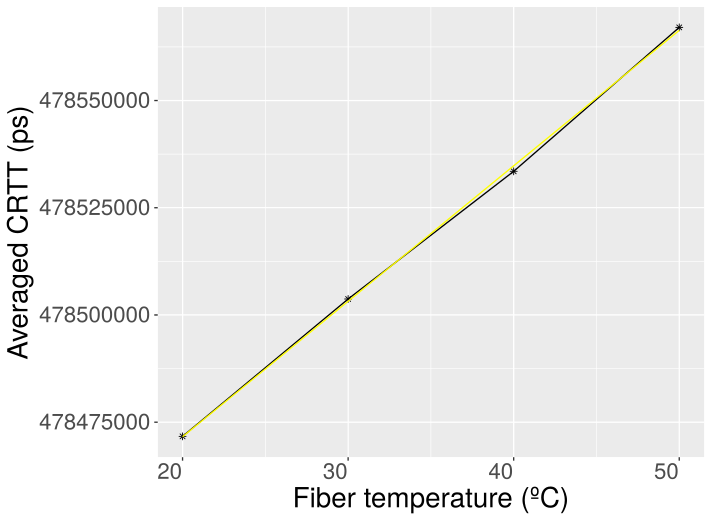
\includegraphics[width=\textwidth]{img/crttvstemp}
		\caption[CRTT vs. Fiber temperature]{The figure shows the relation 
		between the fiber temperature and the cable round-trip time.}
		\label{fig:crttvstemp}
	\end{subfigure}
	~ % This symbol adds a white space between images
	\begin{subfigure}[t]{0.48\textwidth}
		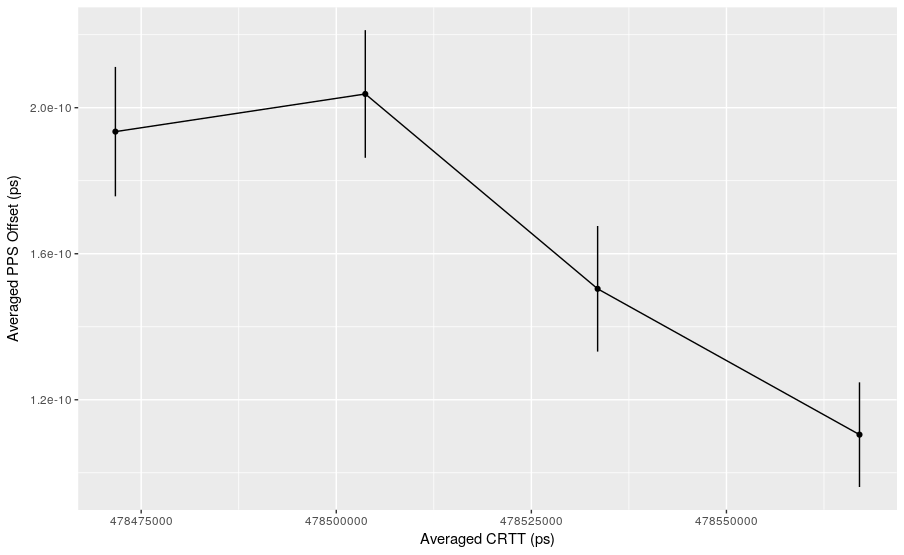
\includegraphics[width=\textwidth]{img/ppsvscrtt}
		\caption[PPS offset vs. CRTT]{This figure shows how PPS offset is 
		sightly influenced by changes in the cable round-trip time.}
		\label{fig:ppsvscrtt}
	\end{subfigure}
\end{figure}
